% Options for packages loaded elsewhere
\PassOptionsToPackage{unicode}{hyperref}
\PassOptionsToPackage{hyphens}{url}
%
\documentclass[
  11pt,
]{article}
\usepackage{amsmath,amssymb}
\usepackage{lmodern}
\usepackage{ifxetex,ifluatex}
\ifnum 0\ifxetex 1\fi\ifluatex 1\fi=0 % if pdftex
  \usepackage[T1]{fontenc}
  \usepackage[utf8]{inputenc}
  \usepackage{textcomp} % provide euro and other symbols
\else % if luatex or xetex
  \usepackage{unicode-math}
  \defaultfontfeatures{Scale=MatchLowercase}
  \defaultfontfeatures[\rmfamily]{Ligatures=TeX,Scale=1}
\fi
% Use upquote if available, for straight quotes in verbatim environments
\IfFileExists{upquote.sty}{\usepackage{upquote}}{}
\IfFileExists{microtype.sty}{% use microtype if available
  \usepackage[]{microtype}
  \UseMicrotypeSet[protrusion]{basicmath} % disable protrusion for tt fonts
}{}
\makeatletter
\@ifundefined{KOMAClassName}{% if non-KOMA class
  \IfFileExists{parskip.sty}{%
    \usepackage{parskip}
  }{% else
    \setlength{\parindent}{0pt}
    \setlength{\parskip}{6pt plus 2pt minus 1pt}}
}{% if KOMA class
  \KOMAoptions{parskip=half}}
\makeatother
\usepackage{xcolor}
\IfFileExists{xurl.sty}{\usepackage{xurl}}{} % add URL line breaks if available
\IfFileExists{bookmark.sty}{\usepackage{bookmark}}{\usepackage{hyperref}}
\hypersetup{
  pdftitle={Estimating survival in left filtered data: simulation and application},
  pdfauthor={Kevin Chen},
  hidelinks,
  pdfcreator={LaTeX via pandoc}}
\urlstyle{same} % disable monospaced font for URLs
\usepackage[margin=2.54cm]{geometry}
\usepackage{graphicx}
\makeatletter
\def\maxwidth{\ifdim\Gin@nat@width>\linewidth\linewidth\else\Gin@nat@width\fi}
\def\maxheight{\ifdim\Gin@nat@height>\textheight\textheight\else\Gin@nat@height\fi}
\makeatother
% Scale images if necessary, so that they will not overflow the page
% margins by default, and it is still possible to overwrite the defaults
% using explicit options in \includegraphics[width, height, ...]{}
\setkeys{Gin}{width=\maxwidth,height=\maxheight,keepaspectratio}
% Set default figure placement to htbp
\makeatletter
\def\fps@figure{htbp}
\makeatother
\setlength{\emergencystretch}{3em} % prevent overfull lines
\providecommand{\tightlist}{%
  \setlength{\itemsep}{0pt}\setlength{\parskip}{0pt}}
\setcounter{secnumdepth}{-\maxdimen} % remove section numbering
\PassOptionsToPackage{no-math}{fontspec}

%---------------------------------------------------------------------------
% Kevin's style file
%---------------------------------------------------------------------------
\usepackage{ifxetex,ifluatex}

%---------------------------------------------------------------------------
% General
%---------------------------------------------------------------------------

% When testing
% \usepackage{lipsum}

% Line numbering
\usepackage{lineno}

% Usage
	% \linenumbers
	% \modulolinenumbers[2]
	% \renewcommand\thelinenumber{\color{red}\Roman{linenumber}}
	% \begin{linenumbers}  \end{linenumbers}


\usepackage{setspace}
%\doublespacing


\usepackage{outlines}
% \usepackage{enumerate}
\usepackage{enumitem} % more powerful than enumerate
% \setenumerate[4]{label=\alph*).}

\setlength\parindent{0pt} % Removes all indentation from paragraphs

\usepackage{sectsty} % Allows customizing section commands
% \renewcommand{\thesection}{\Alph{section}} % Lettered, not numbered sections
% \allsectionsfont{\centering \normalfont\scshape} % Make all sections centered, the default font and small caps
%\numberwithin{equation}{section} % Number equations within sections
%\numberwithin{figure}{section} % Number figures within sections
%\numberwithin{table}{section} % Number tables within sections

\usepackage{multicol}
\setlength{\columnsep}{15pt}
\newlength\Colsep

%---------------------------------------------------------------------------
% Tables, figures, images
%---------------------------------------------------------------------------
\usepackage{color}
% \usepackage[usenames,dvipsnames]{xcolor}
\usepackage{xparse}
\usepackage{xhfill}
\ifnum 0\ifxetex 1\fi\ifluatex 1\fi=0
% Requires pdfTeX
\usepackage{linegoal}
\fi

\usepackage{longtable}
\setlength{\LTcapwidth}{\textwidth}
\usepackage{xtab, booktabs}
\usepackage{multirow}
\usepackage[flushleft]{threeparttable} % Suzanne's

\usepackage{float} % Check code chunks section for floatrow

\usepackage{graphicx}
% \usepackage{grffile}
% \usepackage{subcaption}
% For tables and figures in parts %%%%
\usepackage{caption}
% \DeclareCaptionLabelFormat{cont}{#1~#2\alph{ContinuedFloat}}
% \captionsetup[ContinuedFloat]{labelformat=cont}
%\graphicspath{ {file.path.here} }

% Set column widths in tabular environment!
\usepackage{array}
\newcommand{\PreserveBackslash}[1]{\let\temp=\\#1\let\\=\temp}
\newcolumntype{C}[1]{>{\PreserveBackslash\centering}p{#1}}
\newcolumntype{R}[1]{>{\PreserveBackslash\raggedleft}p{#1}}
\newcolumntype{L}[1]{>{\PreserveBackslash\raggedright}p{#1}}

% STATA output for `estout` package
\def\sym#1{\ifmmode^{#1}\else\(^{#1}\)\fi}

%---------------------------------------------------------------------------
% Header/footer
%---------------------------------------------------------------------------
\usepackage{fancyhdr}
\pagestyle{fancyplain}
\fancyhead[L]{}
\fancyhead[C]{}
\fancyhead[R]{}
% \fancyfoot[L]{}
% \fancyfoot[C]{}
% \fancyfoot[R]{\thepage}
\renewcommand{\headrulewidth}{0pt}
% \renewcommand{\footrulewidth}{0pt}
\setlength{\headheight}{14.5pt}

%---------------------------------------------------------------------------
% Supplement (compatible for Beamer and Article)
%---------------------------------------------------------------------------
\input{\string~/HeadRs/common_supplement.tex}

%---------------------------------------------------------------------------
% Bibliography
%---------------------------------------------------------------------------
% \usepackage[backend=bibtex]{biblatex}

%---------------------------------------------------------------------------
% Usage
%---------------------------------------------------------------------------

% For use in LaTex or Sweave:
% \input{/Users/kevinchen/Documents/computing/HeadRs/StatHead.tex}

% An example YAML header for Rmd
% ---
% title: "Stat 2"
% author: "Kevin Chen"
% date: \today
% output:
%   pdf_document:
%      # keep_tex: true
%     #  pandoc_args: [
%     #   "-V", "classoption=twocolumn"
%     # ]
%      includes:
%         in_header: /Users/kevinchen/Documents/computing/HeadRs/StatHead.tex
% bibliography: /Users/kevinchen/Documents/2017 Fa/245/MV_FinalProj/mv_final.bib
% csl: /Users/kevinchen/Documents/computing/HeadRs/AMA.csl
% geometry: margin=2cm, bottom=2.5cm
% ---


%---------------------------------------------------------------------------
% Fonts
%---------------------------------------------------------------------------

%\usepackage[T1]{fontenc} % Use 8-bit encoding that has 256 glyphs
%\usepackage[utf8]{inputenc}
% Latin Modern Roman
% \usepackage{lmodern}
%\usepackage{fourier} % Use the Adobe Utopia font for the document - comment this line to return to the LaTeX default

\ifluatex
%%%%%%%%%%%%%%%%%%%%%%%%%%%
% For Arial (with lualatex)
%%%%%%%%%%%%%%%%%%%%%%%%%%%
\usepackage[no-math]{fontspec}
% \setmainfont{Arial}[
% % Options below necessary for Windows
% 	% Extension = .ttf,
% 	% UprightFont = *,
% 	% BoldFont = *bd,
% 	% ItalicFont = *i,
% 	% BoldItalicFont = *bi
% 	]
% In YAML
% ---
% mainfont: Arial
% ---
% \usepackage{lualatex-math}

% Math as text, but numerals do not mpa well becuase
% mathastext clahes with unicode-math
% \usepackage[italic]{mathastext}
%%%%%%%%%%%%%%%%%%%%%%%%%%%
\fi
\ifluatex
  \usepackage{selnolig}  % disable illegal ligatures
\fi
\newlength{\cslhangindent}
\setlength{\cslhangindent}{1.5em}
\newlength{\csllabelwidth}
\setlength{\csllabelwidth}{3em}
\newenvironment{CSLReferences}[2] % #1 hanging-ident, #2 entry spacing
 {% don't indent paragraphs
  \setlength{\parindent}{0pt}
  % turn on hanging indent if param 1 is 1
  \ifodd #1 \everypar{\setlength{\hangindent}{\cslhangindent}}\ignorespaces\fi
  % set entry spacing
  \ifnum #2 > 0
  \setlength{\parskip}{#2\baselineskip}
  \fi
 }%
 {}
\usepackage{calc}
\newcommand{\CSLBlock}[1]{#1\hfill\break}
\newcommand{\CSLLeftMargin}[1]{\parbox[t]{\csllabelwidth}{#1}}
\newcommand{\CSLRightInline}[1]{\parbox[t]{\linewidth - \csllabelwidth}{#1}\break}
\newcommand{\CSLIndent}[1]{\hspace{\cslhangindent}#1}

\title{Estimating survival in left filtered data: simulation and
application}
\author{Kevin Chen}
\date{Stat 256: Causal Inference (Fall 2021)}

\begin{document}
\maketitle

\fancyhead[R]{Kevin Chen}
\fancyhead[L]{}
\renewcommand{\headrulewidth}{0pt}

\onehalfspacing
\renewcommand{\arraystretch}{1.1}

\thispagestyle{empty}

\setlength{\columnseprule}{0pt}

\hypertarget{introduction}{%
\section{Introduction}\label{introduction}}

The United Auto Workers-General Motors (UAW-GM) Cohort Study is a
longitudinal occupational cohort study established in the early 1980s to
study the health effects of metalworking fluids (Eisen et al. 1992,
2001). Metalworking fluids (MWF) are complex mixtures of fluids used in
industrial metalworking operations to lubricate and cool machinery and
parts. The three major classes of MWF are straight, soluble, and
synthetic metalworking fluids (Byers 2006). Possible routes of human
exposure include absorption through skin, inhalation or aerosols, and
ingestion of droplets.

A central concern in the analysis of occupational cohorts is the
potential for the healthy worker survivor effect (HWSE), the phenomenon
by which healthy individuals remain at work, while less healthy
individuals leave work -- possibly in response to exposure-related
health decline. In the presence of the HWSE, those with the highest
cumulative occupational exposures are also those who are less at risk of
disease. Thus, standard measures of association would show an inverse
relationship between occupational exposure and poor health outcomes
(Arrighi and Hertz-Picciotto 1994). The HWSE is an example of
time-varying confounding affected by past exposure. Previous studies
have attempted to assess the presence of the HWSE in observed data by
assessing so-called path-specific associations using Cox proportional
hazards modeling (Naimi et al. 2013; Garcia et al. 2017). However, these
measures of associations are themselves subject to the confounding they
seek to quantify.

If sequential ignorability of exposure status at each point in follow-up
and positivity can be attained conditional on covariates, then causal
methods can be applied to account for the HWSE. Past studies have
applied causal methods capable of accounting for time-varying
confounding affected by past exposure to the study of MWF exposures and
cancer mortality outcomes in the UAW-GM Cohort Study (Garcia et al.
2018; Izano et al. 2019), but the study of cancer incidence outcomes is
further problematized by incomplete observation of cancer incidence
outcomes over the study period. We wish to make inferences about the
carcinogenicity of MWF exposure over an individual's lifetime starting
three years after they enter the workforce. The UAW-GM cohort includes
those hired roughly between 1938 and 1982. However, cancer incidence
reporting at the Michigan Cancer Registry did not begin until 1985. In
particular, we have the presence of \emph{left filtering} in the UAW-GM
Cohort Study when cancer incidence is the outcome of interest: before
1985, both cancer incidence status and time of cancer incidence are
unknown. Observation of the complete cancer incidence outcome vector
over the study period is conditional on an individual surviving to 1985
cancer-free.

In the presence of the HWSE, left filtering implies outcome
misclassification that is informative of true cancer status. As part of
her dissertation research, Izano (2017) conducted a quantitative bias
analysis for the estimation of survival curves in the presence of left
filtering and the HWSE. She simulated data compatible with the HWSE and
estimated cancer-free survival curves using an inverse probability of
treatment and censoring weighted Kaplan-Meier (WKM) estimator and the
WKM with an Aalen filter for left-filtering (AWKM) (Andersen et al.
1993; Xie and Liu 2005). Data were simulated under five different
scenarios. The causal estimands of interest were the survival curves
under interventions: (1) always exposed at work with no censoring due to
death and (2) never exposed at work with no censoring due to death. For
each intervention, three survival curves were produced: (1) the true
survival curve, (2) the WKM survival curve, and (3) AWKM survival curve.
The bias in mean survival difference calculated by AWKM was negligible
when the true 20-year risk of cancer was under 0.25.

Here, we replicate the simulation and bias analysis presented in Chapter
3 of Izano (2017), embed the problem in the non-parametric structural
causal approach of Pearl (1995), comment on the results, and apply the
WKM and AWKM estimators to the UAW-GM Cohort.

\hypertarget{methods}{%
\section{Methods}\label{methods}}

\hypertarget{causal-model}{%
\subsection{Causal model}\label{causal-model}}

The UAW-GM Cohort data includes person-year level exposure, outcome, and
covariate data starting three years after hire. To emulate the shape of
the data for this longitudinal cohort, we consider 20 years of data over
time indexed by years since hire. Notation representing the variables of
interest are presented in Table \ref{tab:variables}.

\begin{table}
\caption{Descriptions of variables.}\label{tab:variables}
\begin{center}
\begin{tabular}{lp{0.5\linewidth}}
\toprule
 Variable  &  Description                                 \\ \midrule
 $R$       & Time until start of registry \\
 $W$       & Baseline covariates \\
 $S$       & Susceptibility to effects of metalworking fluid exposure \\
 $H(t)$    & Adverse health status at time $t$ \\
 $N(t)$    & Employment status at time $t$ \\
 $A(t)$    & Metalworking fluid exposure at time $t$ \\
 $D(t)$    & Mortality status at time $t$ \\
 $Y^*(t)$  & Cancer status at time $t$ \\
 $Y(t)$    & Observed Cancer status at time $t$ \\
 $t = \{1, 2, \ldots, 20\}$ & Time, indexed in years after hire \\
 \bottomrule
\end{tabular}
\end{center}\end{table}

Assume we have \(n = 50\,000\) iid units in \(X\) with
\[X_i(t) = \left(R_i = 0, W_i, S_i, \bar H_i(t), \bar N_i(t), \bar A_i(t), \bar a_i(t), \bar Y^*_i(t) = \bar Y_i(t) \right).\]
The bar notation to indicates variable history where
\(\bar X_i(t) = \left(X_i(k)\right)_{k = 1}^t\). In the case of
exposure, \(\bar A_i(t)\) is the indicator of whether unit \(i\) was
ever exposed through time \(t\). Note that true cancer status \(Y^*(t)\)
not observed until \(t \ge R\), after the start of the registry. Call
\(X\) the full data, where we have \(R = 0\) for all. In the observed
data \(X^\text{obs}\), we cannot assume \(R = 0\) for all, and
susceptibility \(S\) is not known:
\[X^\text{obs}_i(t) = \left(R_i, W_i, \bar N_i(t), \bar A_i(t), \bar a_i(t), \bar Y_i(t) \right).\]
Under the causal model, we assume the following non-parametric
structural equations: \[\begin{aligned}
R     & = f_R \left( U_R \right) \\
W     & = f_W \left( U_W \right) \\
S     & = f_S \left( U_S \right) \\
H(t)  & = f_{H(t)} \left( H(t - 1), U_{H(t)} \right) \\
N(t)  & = f_{N(t)} \left( W, N(t - 1), H(t), A(t - 1), U_{N(t)} \right) \\
A(t)  & = f_{A(t)} \left( W, \bar A(t - 1), N(t), U_{A(t)} \right) \\
D(t)  & = f_{D(t)} \left( W, \bar A(t - 1), D(t - 1), Y^*(t - 1), U_{D(t)} \right) \\
Y^*(t)& = f_{Y^*(t)} \left(W, S, H(t), \bar A (t), D(t), Y^*(t - 1), U_{Y^*(t)} \right) \\
Y(t) & = Y^*(t) \times \Ind{Y^*(\lfloor R \rfloor) = 0} \times \Ind{D(t) = 0} \ .
\end{aligned}\] The exogenous variables (errors)
\(U = \left( U_R, U_W, U_S, U_{H(t)}, U_{N(t)}, U_{A(t)}, U_{D(t)}, U_{Y^*(t)} \right)_{t = 1}^{T}\)
are mutually independent. Exposure status is a time-varying indicator;
let exposure history \(\bar A(t)\) be summarized as being ever-exposed
or not with \(\bar A(t) = \Ind{\sum_{k = 1}^t\Ind{A(k) = 1} > 0}\). The
outcome of interest is a survival outcome, so
\(Y^*(t - 1) = 1 \Rightarrow Y^*(t) = 1\). The observed outcome \(Y(t)\)
at time \(t\) is a function of true outcome status and the time points
delimiting left and right censoring. An abbreviated directed acyclic
graph (DAG) representing the causal relationships encoded in the
equations above is presented in Figure \ref{fig:dag}.

\begin{figure}
\caption{Directed acyclic graph representing the causal relationships encoded in the non-parametric structural equation model at time $t$.}
\label{fig:dag}
\begin{center}
\begin{tikzpicture}[>= stealth, auto, node distance = 2.25cm, semithick, fill=white, inner sep=0pt]
\tikzstyle{every state}=[shape = circle, align = center, draw = none]
\node[state] (H0) {$H(t - 1)$};
\node[state] (N0) [below right of=H0] {$N(t - 1)$};
\node[state] (A0) [below right of=N0] {$\bar A(t - 1)$};
\node[state] (D0) [below right of=A0] {$D(t - 1)$};
\node[state] (Y0) [below right of=D0] {$Y^*(t - 1)$};
\node[state] (W) [above right of=H0] {$W$};
\node[state] (H) [right of=H0, node distance = 4cm] {$H(t)$};
\node[state] (N) [below right of=H, node distance = 4cm] {$N(t)$};
\node[state] (A) [below right of=N, node distance = 4cm] {$\bar A(t)$};
\node[state] (D) [above right of=N, node distance = 3cm] {$D(t)$};
\node[state] (Y) [above right of=A, node distance = 3cm] {$Y^*(t)$};
\node[state] (S) [above right of=D, node distance = 3cm] {$S$};
%
\path[->] (H0) edge (H);
\path[->] (W) edge [bend right=10] (N);
\path[->] (N0) edge (N);
\path[->] (H) edge (N);
\path[->] (A0) edge (N);
\path[->] (W) edge [bend right=15] (A);
\path[->] (A0) edge (A);
\path[->] (N) edge (A);
\path[->] (W) edge (D);
\path[->] (A0) edge [bend left=15] (D);
\path[->] (D0) edge [bend right=15] (D);
\path[->] (Y0) edge [bend right=10] (D);
\path[->] (W) edge [bend left=5] (Y);
\path[->] (S) edge [bend left=30] (Y);
\path[->] (S) edge [bend left=15] (Y0);
\path[->] (H) edge (Y);
\path[->] (A) edge (Y);
\path[->] (D) edge (Y);
\path[->] (Y0) edge (Y);
\end{tikzpicture}
\end{center}
\end{figure}

\hypertarget{simulation}{%
\subsection{Simulation}\label{simulation}}

Parametric relationships between the variables were imposed in
simulations. For the \(n = 50\,000\) units over \(T = 20\) years, we
have:

\begin{itemize}
\tightlist
\item
  \(U_j \overset{\text{iid}}{\sim} \text{uniform}\,[0,1]\) for all \(j\)
\item
  In full data \(R = 0\) otherwise \(R \sim \text{uniform}\,[0, 30]\)
\item
  \(W = \Ind{U_W \le p_W} \sim \text{Bernoulli}\left( p_W \right)\)
\item
  \(S = \Ind{U_S \le p_S} \sim \text{Bernoulli}\,(p_S)\)
\item
  If \(H(t - 1) = 1\), then \(H(t) = 1\) otherwise
  \(H(t) = \Ind{U_{H(t)} \le p_H} \sim \text{Bernoulli}\,(p_H)\)
\item
  if \(N(t - 1) = 0\) then \(N(t) = 0\) otherwise
  \[N(t) \sim \text{Bernoulli}\left\{
    \text{logit}\,\left(
        \beta_0^N
        + \beta_W^N W
        + \beta_H^N H(t)
        + \beta_A^N A(t - 1) \times \Ind{t > 1}
        + U_{N(t)}
    \right)
    \right\}\]
\item
  If \(N(t) = 0\) then \(A(t) = 0\) otherwise
  \[A(t) \sim \text{Bernoulli}\left\{
    \text{logit}\,\left(
        \left( \beta_0^A + \beta_W^A W\right) \times \Ind{t = 1}
        + \beta_A^A A(t - 1) \times \Ind{t > 1}
        + U_{A(t)}
    \right)
    \right\}\]
\item
  If \(D(t - 1) = 1\) then \(D(t) = 1\) otherwise
  \[D(t) \sim \text{Bernoulli}\left\{
    \text{logit}\,\left(\begin{aligned}
        \beta_0^D
        + \beta_W^D W
        + \beta_{\bar A}^D \bar A(t - 1) \times \Ind{t > 1} \\
        + \beta_{\bar Y}^D \sum_{k = 1}^{t - 1} Y^*(k) \times \Ind{t > 1}
        + U_{D(t)}
    \end{aligned}\right)
    \right\}\]
\item
  If \(Y^*(t - 1) = 1\) then \(Y^*(t) = 1\) otherwise
  \[Y^*(t) \sim \text{Bernoulli}\left\{
    \text{logit}\,\left(\begin{aligned}
        \beta_0^Y
        + \beta_W^Y W
        + \beta_{A}^Y A(t)
        + \beta_{\bar A}^Y \bar A(t - 1) \times \Ind{t > 1} \\
        + \beta_{S}^Y S \times \bar A(t)
        + \beta_{H}^Y H(t)
        + U_{Y^*(t)}
    \end{aligned}\right)
    \right\}\]
\item
  If \(t < R\) then \(Y(t) = 0\)
\item
  If \(t \ge R\) then
  \(Y(t) = Y^*(t) \times \Ind{Y^*(\lfloor R \rfloor) = 0} \times \Ind{D(t) = 0}\).
\end{itemize}

Five sets of data were generated using these equations to represent five
scenarios. Scenario 1 represents the base case where 10\% of workers are
susceptible to exposure-related effects, the odds ratio of mortality
each additional year following cancer diagnosis is about 1.6, and there
is moderate time-varying confounding by health status. In scenario 2, we
have greater cancer-related mortality by increasing
\(\beta_{\bar Y}^D\). In scenario 3, we increase \(p_S\), the proportion
of the study population susceptible to the carcinogenic effects of MWF
exposure. In scenario 4, we consider greater time-varying confounding by
health status by increasing \(\beta_H^N\) and \(\beta_H^Y\). In the last
scenario, we have greater background cancer incidence by increasing
\(\beta_0^Y\). The sets of parameters used in the five scenarios are
presented in Table \ref{tab:params}.

\begin{table}
\caption{Simulation parameters.}
\label{tab:params}
\begin{center}
\begin{tabular}{rrrrrr}
  \toprule
Parameter & Scenario 1 & Scenario 2 & Scenario 3 & Scenario 4 & Scenario 5 \\ 
  \midrule
$p_S$ & 0.10 & 0.10 & \textbf{0.20} & 0.10 & 0.10 \\ 
  $p_W$ & 0.20 & 0.20 & 0.20 & 0.20 & 0.20 \\ 
  $p_H$ & 0.30 & 0.30 & 0.30 & 0.30 & 0.30 \\ 
  $\beta_0^N$ & 3.00 & 3.00 & 3.00 & 3.00 & 3.00 \\ 
  $\beta_W^N$ & -0.10 & -0.10 & -0.10 & -0.10 & -0.10 \\ 
  $\beta_H^N$ & -0.50 & -0.50 & -0.50 & \textbf{-1.50} & -0.50 \\ 
  $\beta_A^N$ & -1.50 & -1.50 & -1.50 & -1.50 & -1.50 \\ 
  $\beta_0^A$ & -1.50 & -1.50 & -1.50 & -1.50 & -1.50 \\ 
  $\beta_W^A$ & -0.50 & -0.50 & -0.50 & -0.50 & -0.50 \\ 
  $\beta_A^A$ & 2.50 & 2.50 & 2.50 & 2.50 & 2.50 \\ 
  $\beta_0^D$ & -5.50 & -5.50 & -5.50 & -5.50 & -5.50 \\ 
  $\beta_W^D$ & 1.00 & 1.00 & 1.00 & 1.00 & 1.00 \\ 
  $\beta_{\bar A}^D$ & 0.50 & 0.50 & 0.50 & 0.50 & 0.50 \\ 
  $\beta_{\bar Y}^D$ & 0.50 & \textbf{2.00} & 0.50 & 0.50 & 0.50 \\ 
  $\beta_0^Y$ & -7.00 & -7.00 & -7.00 & -7.00 & \textbf{-6.00} \\ 
  $\beta_W^Y$ & 2.00 & 2.00 & 2.00 & 2.00 & 2.00 \\ 
  $\beta_A^Y$ & 0.25 & 0.25 & 0.25 & 0.25 & 0.25 \\ 
  $\beta_{\bar A}^Y$ & 0.20 & 0.20 & 0.20 & 0.20 & 0.20 \\ 
  $\beta_H^Y$ & 0.70 & 0.70 & 0.70 & \textbf{1.70} & 0.70 \\ 
  $\beta_S^Y$ & 0.30 & 0.30 & 0.30 & 0.30 & 0.30 \\ 
   \bottomrule
\end{tabular}
\end{center}
\end{table}

\hypertarget{interventions-potential-outcomes-target-parameters-and-estimation}{%
\subsection{Interventions, potential outcomes, target parameters, and
estimation}\label{interventions-potential-outcomes-target-parameters-and-estimation}}

The substantive question of interest is the causal effect of
occupational exposure to MWF on cancer incidence risk. Since
occupational MWF exposure occurs only when individuals are at work, we
define dynamic exposure regimes that depend on employment status. Under
rule \(a_0\), set \(D(t) = 0\), and set \(A(t) = 0\) while \(N(t) = 1\).
Under rule \(a_1\), set \(D(t) = 0\), and set \(A(t) = 1\) while
\(N(t) = 1\). Under both rules, we prevent censoring by death as if it
were intervenable. The causal effect is defined by contrasting the
survival function \(S_{a_1}(t) = 1 - \E{Y_{a_1}(t)}\) under rule \(a_1\)
to \(S_{a_0}(t) = 1 - \E{Y_{a_0}(t)}\) that under rule \(a_0\). Note
that this causal estimand is defined over \emph{a priori
counterfactuals} not observable in the real world (Frangakis and Rubin
2002). This approach is standard in epidemiologic studies, however.

The survival function expresses the probability that a person following
rule \(a\) is cancer-free at the end of time point \(t\). The expected
time until cancer under rule \(a\) is
\(\mu_{a} = \sum_0^K S_{a}(t) \, dt\). Our causal estimand is summary
measure \(\psi = \mu_{a_1} - \mu_{a_0}\), the difference in expected
time until event under two different interventions over 20 years of
follow-up under five different data generating scenarios. Bias will be
evaluated by comparing estimates of \(\psi\) to its true value in 250
simulations per scenario (the original analysis performed 500). The true
value will be calculated by simulating the full data for five hundred
thousand individuals (the original analysis used one million) with rules
\(a_0\) and \(a_1\) applied deterministically. Estimates of \(\psi\)
will be obtained by first estimating the survival curves \(S_a(t)\)
using two estimators: the inverse probability weighted Kaplan-Meier
estimator (WKM) and the Aalen-filtered WKM (AWKM). These survival
estimators are detailed in the following section.

\hypertarget{kaplan-meier-estimator-and-extensions}{%
\subsection{Kaplan-Meier estimator and
extensions}\label{kaplan-meier-estimator-and-extensions}}

To estimate survival, we applied extensions of the widely-known
Kaplan-Meier (KM) estimator for survival (Kaplan and Meier 1958). First,
we review the estimator of Xie and Liu (2005), an extension of the KM
estimator where units are weighted by the inverse probability of
treatment. The standard KM estimator requires counting up the number of
cases \(c^0_{a}(t)\) that occurred in interval \((t - 1, t]\) and the
number of units at risk \(R^0_{a}(t)\) in that interval at all event
times \(t\). Assuming cancer status was assessed at the end of regular
intervals \(t = 1, \ldots, K\), we have: \[\begin{aligned}
c^0_{a} (t)
& = \sum_i^n \Ind{Y_i(t) = 1} \times \Ind{Y_i(t - 1) = 0} \times \Ind{\bar A_i (t) = \bar a(t)} \\
R^0_{a} (t)
& = \sum_i^n \Ind{Y_i(t - 1) = 0} \times \Ind{\bar A_i (t) = \bar a(t)}.
\end{aligned}\] The standard survival estimator is \[\hat S^0_{a}(t) =
\begin{cases}
1 & \text{if } t < t_1 \\
\prod_{j \le t} \left(1 - \frac{c^0_{a}(j)}{R^0_{a}(j)}\right) & \text{if } t \ge t_1 \\
\end{cases}\] where \(t_1\) is the first event time.

In observational studies, survival contrasts estimated using the
standard KM estimator are biased for the true causal survival contrast.
However, if conditional ignorability and positivity are attained, the
inverse probability weighted KM (WKM) estimator of Xie and Liu (2005)
yields unbiased estimates of the true causal survival curve. The WKM
estimator augments the standard KM estimator by weighting units at time
\(t\) by \(w_{i, a}(t)\) the inverse probability of treatment:
\[\begin{aligned}
c^w_{a} (t)
& = \sum_i^n w_{i, a}(t) \times \Ind{Y_i(t) = 1} \times \Ind{Y_i(t - 1) = 0} \times \Ind{\bar A_i (t) = \bar a(t)}\\
R^w_{a} (t)
& = \sum_i^n w_{i, a}(t) \times \Ind{Y_i(t - 1) = 0} \times \Ind{\bar A_i (t) = \bar a(t)}
\end{aligned}\] The WKM survival estimator for rule \(a\) is
\[\hat S^w_{a}(t) =
\begin{cases}
1 & \text{if } t < t_1 \\
\prod_{j \le t} \left(1 - \frac{c^w_{a}(j)}{R^w_{a}(j)}\right) & \text{if } t \ge t_1 \\
\end{cases}\] where \(t_1\) is the first event time.

Finally, to account for (uninformative) left filtering, we applied the
Aalen filter, which considers only the units at time \(t\) for which the
outcome is observed: \[\begin{aligned}
c_{a} (t)
& = \sum_i^n w_{i, a}(t) \times \Ind{Y_i(t) = 1} \times \Ind{Y_i(t - 1) = 0} \times \Ind{\bar A_i (t) = \bar a(t)} \times \Ind{t \ge R_i} \\
R_{a} (t)
& = \sum_i^n w_{i, a}(t) \times \Ind{Y_i(t - 1) = 0} \times \Ind{\bar A_i (t) = \bar a(t)} \times \Ind{t \ge R_i}
\end{aligned}\] The Aalen-filtered WKM (AWKM) estimator for rule \(a\)
is \[\hat S_{a}(t) =
\begin{cases}
1 & \text{if } t < t_1 \\
\prod_{j \le t} \left(1 - \frac{c_{a}(j)}{R_{a}(j)}\right) & \text{if } t \ge t_1 \\
\end{cases}\] where \(t_1\) is the first event time.

In the full data, the WKM and AWKM estimators are equivalent, and
identification is achieved under overlap (positivity) and sequential
ignorability (randomization) assumptions: \[\begin{aligned}
Y^*_{a, \bar d = 0} (t')   & \indep A(t) \mid W,\ \bar A(t - 1) = \bar a(t - 1),\ D(t - 1) = 0,\ N(t) = 1\\
Y^*_{a, \bar d = 0} (t') & \indep D(t) \mid W,\ D(t - 1) = 0,\ Y^*(t - 1) = 0,\ \bar A(t - 1) = \bar a(t - 1)
\end{aligned}\] for all times \(t'\ge t\), and
\[0 < \Prob{ A(t) = 1 \mid W,\ \bar A(t - 1) = \bar a(t - 1),\ D(t - 1) = 0,\ N(t) = 1} < 1\]
\[0 < \Prob{D(t) = 0 \mid W,\ D(t - 1) = 0,\ Y^*(t - 1) = 0,\ \bar A(t - 1) = \bar a(t - 1)} < 1.\]

Graphical representations of the first and second components of the
ignorability assumption are presented in Figures
\ref{fig:ignorability_a} and \ref{fig:ignorability_d} where conditioning
on boxed variables are represented by the removal of edges pointing away
from those variables. The resulting graphs show the fulfillment of
Pearl's backdoor criterion for the estimation of the causal effects of
\(\bar A(t)\) on \(Y^*(t)\) and \(D(t)\) on \(Y^*(t)\), respectively.
Thus, the causal effect of the joint intervention on
\(\big(\bar A(t), D(t)\big)\) at each time \(t\) is identified. Causal
identification is not attained when true cancer status \(Y^*(t)\) is not
known.

\begin{figure}
\caption{Directed acyclic graph representing the causal relationships encoded in the non-parametric structural equation model at time $t$ after conditioning on $\{W,\ \bar A(t - 1),\ D(t - 1),\ N(t)\}$.}
\label{fig:ignorability_a}
\begin{center}
\begin{tikzpicture}[>= stealth, auto, node distance = 2.25cm, semithick, fill=white, inner sep=0pt]
\tikzstyle{every state}=[shape = circle, align = center, draw = none]
\node[state] (H0) {$H(t - 1)$};
\node[state] (N0) [below right of=H0] {$N(t - 1)$};
\node[state] (A0) [shape=rectangle, draw=black, inner sep=2.5pt, below right of=N0] {$\bar A(t - 1)$};
\node[state] (D0) [shape=rectangle, draw=black, inner sep=2.5pt, below right of=A0] {$D(t - 1)$};
\node[state] (Y0) [below right of=D0] {$Y^*(t - 1)$};
\node[state] (W) [shape=rectangle, draw=black, inner sep=2.5pt, above right of=H0] {$W$};
\node[state] (H) [right of=H0, node distance = 4cm] {$H(t)$};
\node[state] (N) [shape=rectangle, draw=black, inner sep=2.5pt, below right of=H, node distance = 4cm] {$N(t)$};
\node[state] (A) [below right of=N, node distance = 4cm] {$\bar A(t)$};
\node[state] (D) [above right of=N, node distance = 3cm] {$D(t)$};
\node[state] (Y) [above right of=A, node distance = 3cm] {$Y^*(t)$};
\node[state] (S) [above right of=D, node distance = 3cm] {$S$};
%
\path[->] (H0) edge (H);
\path[->] (N0) edge (N);
\path[->] (H) edge (N);
\path[->] (S) edge [bend left=15] (Y0);
\path[->] (S) edge [bend left=30] (Y);
\path[->] (H) edge (Y);
\path[->] (A) edge (Y);
\path[->] (D) edge (Y);
\path[->] (Y0) edge [bend right=10] (D);
\path[->] (Y0) edge (Y);
\end{tikzpicture}
\end{center}
\end{figure}

\begin{figure}
\caption{Directed acyclic graph representing the causal relationships encoded in the non-parametric structural equation model at time $t$ after conditioning on $\{W,\ \bar A(t - 1),\ D(t - 1),\ Y^*(t - 1)\}$.}
\label{fig:ignorability_d}
\begin{center}
\begin{tikzpicture}[>= stealth, auto, node distance = 2.25cm, semithick, fill=white, inner sep=0pt]
\tikzstyle{every state}=[shape = circle, align = center, draw = none]
\node[state] (H0) {$H(t - 1)$};
\node[state] (N0) [below right of=H0] {$N(t - 1)$};
\node[state] (A0) [shape=rectangle, draw=black, inner sep=2pt, below right of=N0] {$\bar A(t - 1)$};
\node[state] (D0) [shape=rectangle, draw=black, inner sep=2pt, below right of=A0] {$D(t - 1)$};
\node[state] (Y0) [shape=rectangle, draw=black, inner sep=2pt, below right of=D0] {$Y^*(t - 1)$};
\node[state] (W) [shape=rectangle, draw=black, inner sep=2pt, above right of=H0] {$W$};
\node[state] (H) [right of=H0, node distance = 4cm] {$H(t)$};
\node[state] (N) [below right of=H, node distance = 4cm] {$N(t)$};
\node[state] (A) [below right of=N, node distance = 4cm] {$\bar A(t)$};
\node[state] (D) [above right of=N, node distance = 3cm] {$D(t)$};
\node[state] (Y) [above right of=A, node distance = 3cm] {$Y^*(t)$};
\node[state] (S) [above right of=D, node distance = 3cm] {$S$};
%
\path[->] (H0) edge (H);
%\path[->] (W) edge [bend right=10] (N);
\path[->] (N0) edge (N);
\path[->] (H) edge (N);
%\path[->] (A0) edge (N);
%\path[->] (W) edge [bend right=15] (A);
%\path[->] (A0) edge (A);
\path[->] (N) edge (A);
%\path[->] (W) edge (D);
%\path[->] (A0) edge [bend left=15] (D);
%\path[->] (D0) edge [bend right=15] (D);
%\path[->] (Y0) edge [bend right=10] (D);
%\path[->] (W) edge [bend left=5] (Y);
\path[->] (S) edge [bend left=30] (Y);
\path[->] (S) edge [bend left=15] (Y0);
\path[->] (H) edge (Y);
\path[->] (A) edge (Y);
\path[->] (D) edge (Y);
%\path[->] (Y0) edge (Y);
\end{tikzpicture}
\end{center}
\end{figure}

\hypertarget{estimation-of-weights}{%
\subsection{Estimation of weights}\label{estimation-of-weights}}

To estimate the weights for the WKM and AWKM estimators, we fit two
logistic regressions at each time point \(t = 1, \ldots 20\):
\[\begin{aligned}
\text{logit} \left(\Prob{
    A(t) = 1
    \mid W,\ \bar A(t - 1),\ D(t - 1) = 0,\ N(t) = 1
    }\right)
& = \alpha_0 + W \alpha_1 + \bar A(t - 1) \alpha_2 \\
\text{logit} \left(\Prob{
    D(t) = 1
    \mid W,\ D(t - 1) = 0,\ Y(t - 1) = 0,\ \bar A(t - 1)}\right)
    & = \beta_0 + W \beta_1 + \bar A(t - 1) \beta_2
\end{aligned}\] The first will be fitted on data for those alive and at
work at time \(t\). The second will be among those alive and (observed
to be) cancer-free. For each unit at time \(t\), the weight will be
calculated by taking the inverse of the cumulative probability of
following the exposure rule and remaining uncensored: \[\hat w_{a} (t) =
    \left[
    \prod^t_{j = 1}
    \begin{aligned}
    \widehat {\mathbb P} \left\{
    A(j) = a(j) \mid W,\ \bar A(j - 1) = \bar a (j - 1),\ D(j - 1) = 0,\ N(j) = 1
    \right\} \times \\
    \widehat {\mathbb P} \left\{D(j) = 0
    \mid W,\ D(j - 1) = 0,\ Y(j - 1) = 0,\ \bar A(j) = \bar a (j) \right\}
    \end{aligned}\right]^{-1}.\]

\hypertarget{results}{%
\section{Results}\label{results}}

Figure \ref{fig:survival} presents the true survival curves as well as
the WKM and AWKM survival curves averaged over 250 replications for each
intervention rule and scenario. Qualitatively, the WKM estimator
consistently over-estimates survival whereas the the AWKM survival curve
is much closer to the truth. The bias of the AWKM survival estimate
appears to be larger earlier in follow-up and smaller as follow-up
extends forward. The bias of both the the WKM and the AWKM survival
curves appears largest in Scenario 5.

\begin{figure}
\caption{Cancer-free survival over time since hire in five simulation scenarios. The true (discrete) survival curve is represented by the solid lines. The average inverse probability weighted Kaplan-Meier (WKM) survival curve is represented by the dashed-line with short dashes. The average Aalen-filtered inverse probability weighted Kaplan-Meier (AWKM) survival curve is represented by the dashed-line with long dashes. Estimated survival curves were averaged over 250 replicates. Salmon color indicates survival and survival estimates under rule $a_0$ when workers are always unexposed. Cyan color indicates those under rule $a_1$ when workers are always exposed while employed.}
\label{fig:survival}
\begin{center}
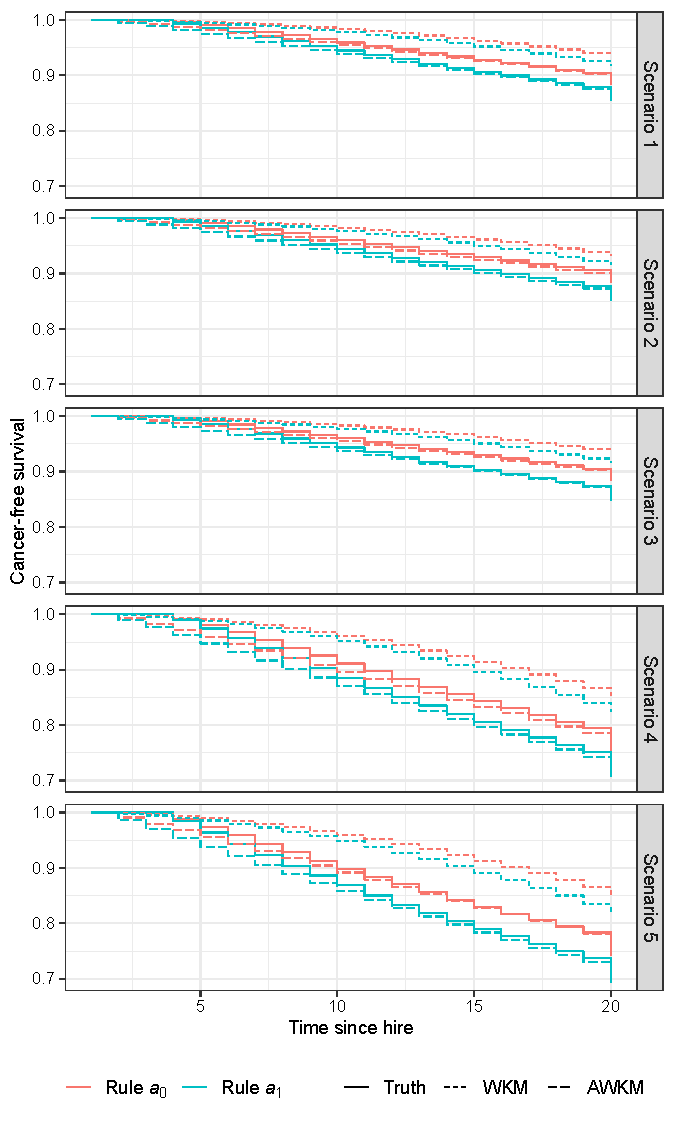
\includegraphics{/Users/kevinchen/Documents/2021 Fall/256 - Causal Inference/256-final/reports/resources/results.pdf}
\end{center}
\end{figure}

Table \ref{tab:survival} presents true and estimated average cancer-free
survival times under each intervention rule and scenario. Table
\ref{tab:differences} presents differences in survival time contrasting
rule \(a_1\) to rule \(a_0\). Table \ref{tab:bias} presents estimates of
the bias of the WKM and AWKM estimators for \(\psi\), the difference in
average cancer-free survival time over 20 years of follow-up. These
numeric results are consistent with the qualitative interpretations of
Figure \ref{fig:survival}. The WKM estimator over-estimates the
difference in cancer-free survival time, resulting in bias toward the
null, whereas the AWKM estimator under-estimates the cancer-free
survival, resulting in bias away from the null. In every scenario, the
bias of the WKM-derived contrast is several times larger in magnitude
than that of the AWKM-derived contrast. The bias of both estimators is
greatest for Scenario 5.

The qualitative results here are consistent with those of Izano (2017).
However, true and estimated survival in the present analysis is larger
than those found previously. Furthermore, the true and estimator average
mean differences in survival are smaller in magnitude in the present
case. The magnitudes of the bias estimates are also smaller.

\begin{table}[H]
\centering
\caption{True cancer-free survival time $\mu_{a}$ over 20-year follow-up and estimator averages over 250 replicates.} 
\label{tab:survival}
\begin{tabular}{llrrrrr}
  \toprule
Rule & Estimator & Scenario 1 & Scenario 2 & Scenario 3 & Scenario 4 & Scenario 5 \\ 
  \midrule
$a_0$ & Truth & 19.08 & 19.10 & 19.10 & 18.02 & 17.83 \\ 
   & WKM & 19.52 & 19.51 & 19.53 & 18.92 & 18.90 \\ 
   & AWKM & 19.02 & 19.00 & 19.02 & 17.79 & 17.72 \\ 
   \midrule
$a_1$ & Truth & 18.80 & 18.79 & 18.76 & 17.54 & 17.29 \\ 
   & WKM & 19.39 & 19.37 & 19.37 & 18.68 & 18.62 \\ 
   & AWKM & 18.70 & 18.67 & 18.67 & 17.30 & 17.07 \\ 
   \bottomrule
\end{tabular}
\end{table}
\begin{table}[H]
\centering
\caption{Difference in average cancer-free survival time over 20-year follow-up comparing rule $a_1$ always exposed to rule $a_0$ never exposed at work: true value $\psi$ and estimator averages over 250 replicates.} 
\label{tab:differences}
\begin{tabular}{lrrrrr}
  \toprule
Estimator & Scenario 1 & Scenario 2 & Scenario 3 & Scenario 4 & Scenario 5 \\ 
  \midrule
Truth & -0.28 & -0.31 & -0.34 & -0.48 & -0.54 \\ 
  WKM & -0.14 & -0.15 & -0.15 & -0.23 & -0.28 \\ 
  AWKM & -0.31 & -0.33 & -0.35 & -0.50 & -0.64 \\ 
   \bottomrule
\end{tabular}
\end{table}
\begin{table}[H]
\centering
\caption{Bias estimates of estimators for $\psi$, the difference in average cancer-free survival time over 20 years of follow-up.} 
\label{tab:bias}
\begin{tabular}{lrrrrr}
  \toprule
Estimator & Scenario 1 & Scenario 2 & Scenario 3 & Scenario 4 & Scenario 5 \\ 
  \midrule
WKM & 0.14 & 0.16 & 0.19 & 0.25 & 0.26 \\ 
  AWKM & -0.03 & -0.02 & -0.01 & -0.02 & -0.10 \\ 
   \bottomrule
\end{tabular}
\end{table}

\newpage

\hypertarget{references}{%
\section*{References}\label{references}}
\addcontentsline{toc}{section}{References}

\hypertarget{refs}{}
\begin{CSLReferences}{1}{0}
\leavevmode\hypertarget{ref-Andersen_1993}{}%
Andersen, P. K., Ø. Borgan, R. D. Gill, and N. Keiding. 1993.
\emph{Statistical Models Based on Counting Processes}. Springer Series
in Statistics. Springer, New York, NY.
\url{https://books.google.com/books?id=kBnvAAAAMAAJ}.

\leavevmode\hypertarget{ref-Arrighi_1994}{}%
Arrighi, H. Michael, and Irva Hertz-Picciotto. 1994. {``The Evolving
Concept of the Healthy Worker Survivor Effect.''} \emph{Epidemiology} 5
(2): 189--96. \url{http://www.jstor.org/stable/3702361}.

\leavevmode\hypertarget{ref-Byers_2006}{}%
Byers, Jerry P. 2006. \emph{Metalworking Fluids}. CRC Press.

\leavevmode\hypertarget{ref-Eisen_2001}{}%
Eisen, Ellen A, Judith Bardin, Rebecca Gore, Susan R Woskie, Marilyn F
Hallock, and Richard R Monson. 2001. {``Exposure-Response Models Based
on Extended Follow-up of a Cohort Mortality Study in the Automobile
Industry.''} \emph{Scandinavian Journal of Work, Environment \& Health}
27 (4): 240--49.

\leavevmode\hypertarget{ref-Eisen_1992}{}%
Eisen, Ellen A, Paige E Tolbert, Richard R Monson, and Thomas J Smith.
1992. {``Mortality Studies of Machining Fluid Exposure in the Automobile
Industry {I}: A Standardized Mortality Ratio Analysis.''} \emph{American
Journal of Industrial Medicine} 22 (6): 809--24.

\leavevmode\hypertarget{ref-Frangakis_2002}{}%
Frangakis, Constantine E, and Donald B Rubin. 2002. {``Principal
Stratification in Causal Inference.''} \emph{Biometrics} 58 (1): 21--29.

\leavevmode\hypertarget{ref-Garcia_2017}{}%
Garcia, Erika, Sally Picciotto, Sadie Costello, Patrick T Bradshaw, and
Ellen A Eisen. 2017. {``Assessment of the Healthy Worker Survivor Effect
in Cancer Studies of the United Autoworkers-General Motors Cohort.''}
\emph{Occupational and Environmental Medicine} 74 (4): 294--300.

\leavevmode\hypertarget{ref-Garcia_2018}{}%
Garcia, Erika, Sally Picciotto, Andreas M Neophytou, Patrick T Bradshaw,
John R Balmes, and Ellen A Eisen. 2018. {``Lung Cancer Mortality and
Exposure to Synthetic Metalworking Fluid and Biocides: Controlling for
the Healthy Worker Survivor Effect.''} \emph{Occupational and
Environmental Medicine} 75 (10): 730--35.

\leavevmode\hypertarget{ref-Izano_2017_thesis}{}%
Izano, Monika A. 2017. {``Estimating Causal Effects of Occupational
Exposures.''} PhD thesis, University of California, Berkeley; University
of California, Berkeley.

\leavevmode\hypertarget{ref-Izano_2019}{}%
Izano, Monika A, Oleg A Sofrygin, Sally Picciotto, Patrick T Bradshaw,
and Ellen A Eisen. 2019. {``Metalworking Fluids and Colon Cancer Risk:
Longitudinal Targeted Minimum Loss-Based Estimation.''}
\emph{Environmental Epidemiology} 3 (1): e035.

\leavevmode\hypertarget{ref-Kaplan_1958}{}%
Kaplan, Edward L, and Paul Meier. 1958. {``Nonparametric Estimation from
Incomplete Observations.''} \emph{Journal of the American Statistical
Association} 53 (282): 457--81.

\leavevmode\hypertarget{ref-Naimi_2013}{}%
Naimi, Ashley I, Stephen R Cole, Michael G Hudgens, M Alan Brookhart,
and David B Richardson. 2013. {``Assessing the Component Associations of
the Healthy Worker Survivor Bias: Occupational Asbestos Exposure and
Lung Cancer Mortality.''} \emph{Annals of Epidemiology} 23 (6): 334--41.

\leavevmode\hypertarget{ref-Pearl_1995}{}%
Pearl, Judea. 1995. {``Causal Diagrams for Empirical Research.''}
\emph{Biometrika} 82 (4): 669--88.

\leavevmode\hypertarget{ref-Xie_2005}{}%
Xie, Jun, and Chaofeng Liu. 2005. {``Adjusted Kaplan--Meier Estimator
and Log-Rank Test with Inverse Probability of Treatment Weighting for
Survival Data.''} \emph{Statistics in Medicine} 24 (20): 3089--3110.

\end{CSLReferences}

\end{document}
